\documentclass{standalone}
\usepackage{tikz}
\usetikzlibrary{patterns, positioning}


\begin{document}
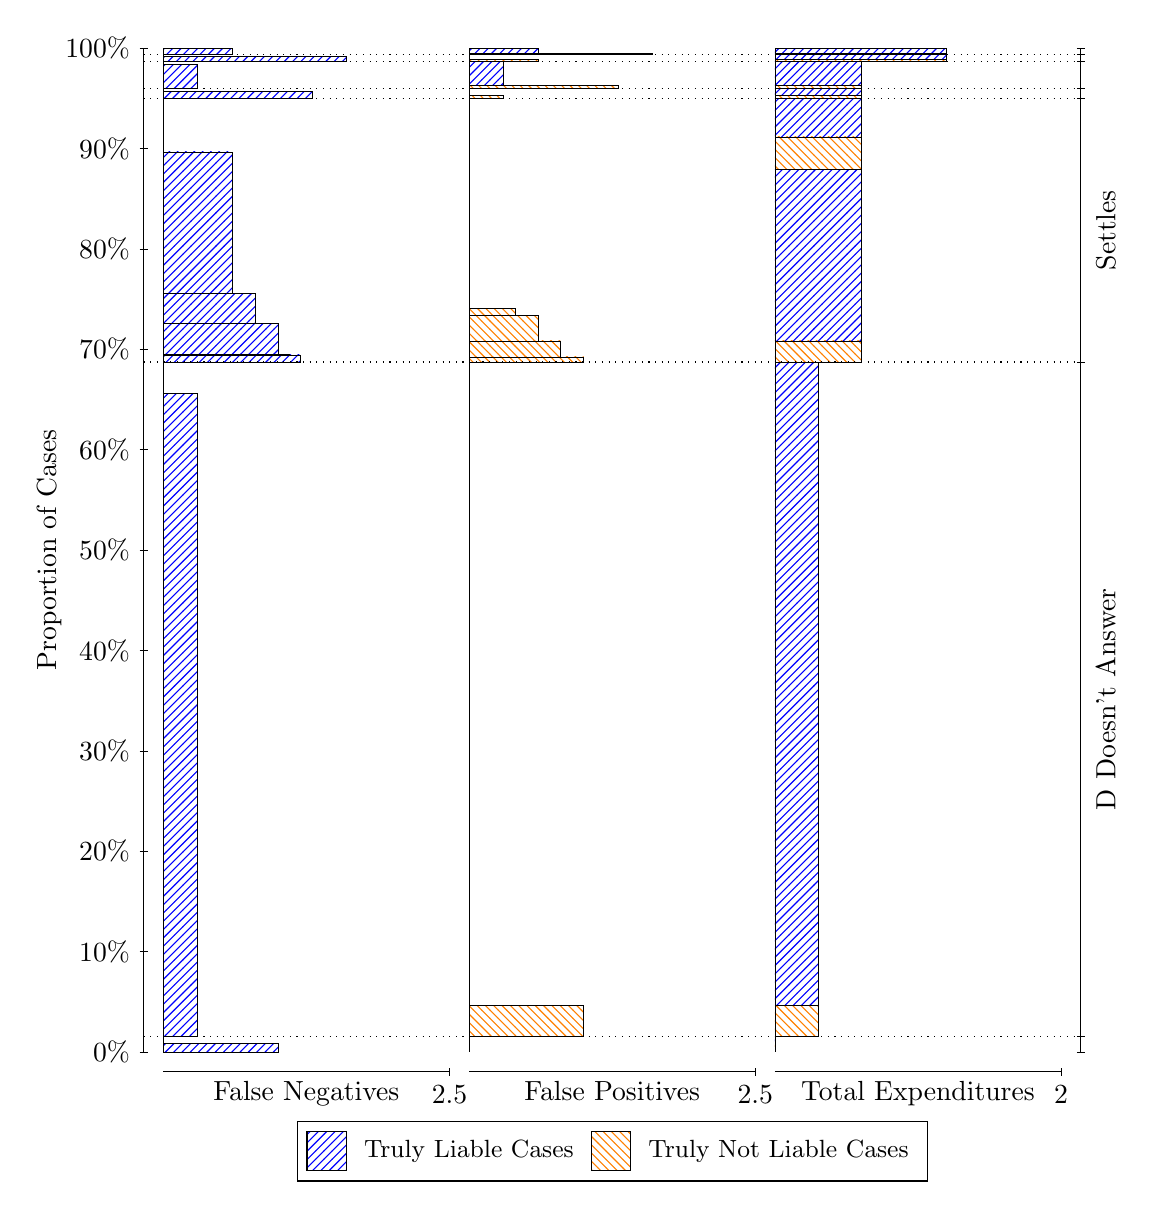
\begin{tikzpicture}
\draw[black, very thin] (1.5,1.75) -- (1.5,14.5);
\node[rotate=90, text=black, anchor=center] at (0.3, 8.125) {Proportion of Cases};
\draw[black, very thin] (1.45,1.75) -- (1.55,1.75);
\node[text=black, anchor=east] at (1.45, 1.75) {0\%};
\draw[black, very thin] (1.45,3.025) -- (1.55,3.025);
\node[text=black, anchor=east] at (1.45, 3.025) {10\%};
\draw[black, very thin] (1.45,4.3) -- (1.55,4.3);
\node[text=black, anchor=east] at (1.45, 4.3) {20\%};
\draw[black, very thin] (1.45,5.575) -- (1.55,5.575);
\node[text=black, anchor=east] at (1.45, 5.575) {30\%};
\draw[black, very thin] (1.45,6.85) -- (1.55,6.85);
\node[text=black, anchor=east] at (1.45, 6.85) {40\%};
\draw[black, very thin] (1.45,8.125) -- (1.55,8.125);
\node[text=black, anchor=east] at (1.45, 8.125) {50\%};
\draw[black, very thin] (1.45,9.4) -- (1.55,9.4);
\node[text=black, anchor=east] at (1.45, 9.4) {60\%};
\draw[black, very thin] (1.45,10.675) -- (1.55,10.675);
\node[text=black, anchor=east] at (1.45, 10.675) {70\%};
\draw[black, very thin] (1.45,11.95) -- (1.55,11.95);
\node[text=black, anchor=east] at (1.45, 11.95) {80\%};
\draw[black, very thin] (1.45,13.225) -- (1.55,13.225);
\node[text=black, anchor=east] at (1.45, 13.225) {90\%};
\draw[black, very thin] (1.45,14.5) -- (1.55,14.5);
\node[text=black, anchor=east] at (1.45, 14.5) {100\%};

\draw[black, very thin] (13.4,1.75) -- (13.4,14.5);
\draw[black, very thin] (13.35,1.75) -- (13.45,1.75);
\node[anchor=west] at (13.35, 1.75) {};
\draw[black, very thin] (13.35,1.9479) -- (13.45,1.9479);
\node[anchor=west] at (13.35, 1.9479) {};
\draw[black, very thin] (13.35,10.512) -- (13.45,10.512);
\node[anchor=west] at (13.35, 10.512) {};
\draw[black, very thin] (13.35,13.86) -- (13.45,13.86);
\node[anchor=west] at (13.35, 13.86) {};
\draw[black, very thin] (13.35,13.984) -- (13.45,13.984);
\node[anchor=west] at (13.35, 13.984) {};
\draw[black, very thin] (13.35,14.326) -- (13.45,14.326);
\node[anchor=west] at (13.35, 14.326) {};
\draw[black, very thin] (13.35,14.42) -- (13.45,14.42);
\node[anchor=west] at (13.35, 14.42) {};
\draw[black, very thin] (13.35,14.5) -- (13.45,14.5);
\node[anchor=west] at (13.35, 14.5) {};

\draw[black, very thin, pattern color=blue, pattern=north east lines] (1.75,1.75) rectangle (3.2033,1.8591);
\draw[black, very thin, pattern color=orange, pattern=north west lines] (1.75,1.8591) rectangle (1.75,1.9479);
\draw[black, very thin, pattern color=blue, pattern=north east lines] (1.75,1.9479) rectangle (2.186,10.115);
\draw[black, very thin, pattern color=orange, pattern=north west lines] (1.75,10.115) rectangle (1.75,10.512);
\draw[black, very thin, pattern color=blue, pattern=north east lines] (1.75,10.512) rectangle (3.494,10.602);
\draw[black, very thin, pattern color=blue, pattern=north east lines] (1.75,10.602) rectangle (3.3487,10.608);
\draw[black, very thin, pattern color=blue, pattern=north east lines] (1.75,10.608) rectangle (3.2033,11.001);
\draw[black, very thin, pattern color=blue, pattern=north east lines] (1.75,11.001) rectangle (2.9127,11.383);
\draw[black, very thin, pattern color=blue, pattern=north east lines] (1.75,11.383) rectangle (2.622,13.181);
\draw[black, very thin, pattern color=orange, pattern=north west lines] (1.75,13.181) rectangle (1.75,13.86);
\draw[black, very thin, pattern color=blue, pattern=north east lines] (1.75,13.86) rectangle (3.6393,13.946);
\draw[black, very thin, pattern color=orange, pattern=north west lines] (1.75,13.946) rectangle (1.75,13.984);
\draw[black, very thin, pattern color=blue, pattern=north east lines] (1.75,13.984) rectangle (2.186,14.288);
\draw[black, very thin, pattern color=orange, pattern=north west lines] (1.75,14.288) rectangle (1.75,14.326);
\draw[black, very thin, pattern color=blue, pattern=north east lines] (1.75,14.326) rectangle (4.0753,14.393);
\draw[black, very thin, pattern color=orange, pattern=north west lines] (1.75,14.393) rectangle (1.75,14.42);
\draw[black, very thin, pattern color=blue, pattern=north east lines] (1.75,14.42) rectangle (2.622,14.493);
\draw[black, very thin, pattern color=orange, pattern=north west lines] (1.75,14.493) rectangle (1.75,14.5);
\draw[black, very thin, pattern color=orange, pattern=north west lines] (5.6333,1.75) rectangle (5.6333,1.8388);
\draw[black, very thin, pattern color=blue, pattern=north east lines] (5.6333,1.8388) rectangle (5.6333,1.9479);
\draw[black, very thin, pattern color=orange, pattern=north west lines] (5.6333,1.9479) rectangle (7.0867,2.3449);
\draw[black, very thin, pattern color=blue, pattern=north east lines] (5.6333,2.3449) rectangle (5.6333,10.512);
\draw[black, very thin, pattern color=orange, pattern=north west lines] (5.6333,10.512) rectangle (7.0867,10.577);
\draw[black, very thin, pattern color=orange, pattern=north west lines] (5.6333,10.577) rectangle (6.796,10.781);
\draw[black, very thin, pattern color=orange, pattern=north west lines] (5.6333,10.781) rectangle (6.5053,11.102);
\draw[black, very thin, pattern color=orange, pattern=north west lines] (5.6333,11.102) rectangle (6.36,11.106);
\draw[black, very thin, pattern color=orange, pattern=north west lines] (5.6333,11.106) rectangle (6.2147,11.19);
\draw[black, very thin, pattern color=blue, pattern=north east lines] (5.6333,11.19) rectangle (5.6333,13.86);
\draw[black, very thin, pattern color=orange, pattern=north west lines] (5.6333,13.86) rectangle (6.0693,13.898);
\draw[black, very thin, pattern color=blue, pattern=north east lines] (5.6333,13.898) rectangle (5.6333,13.984);
\draw[black, very thin, pattern color=orange, pattern=north west lines] (5.6333,13.984) rectangle (7.5227,14.022);
\draw[black, very thin, pattern color=blue, pattern=north east lines] (5.6333,14.022) rectangle (6.0693,14.326);
\draw[black, very thin, pattern color=orange, pattern=north west lines] (5.6333,14.326) rectangle (6.5053,14.353);
\draw[black, very thin, pattern color=blue, pattern=north east lines] (5.6333,14.353) rectangle (5.6333,14.42);
\draw[black, very thin, pattern color=orange, pattern=north west lines] (5.6333,14.42) rectangle (7.9587,14.428);
\draw[black, very thin, pattern color=blue, pattern=north east lines] (5.6333,14.428) rectangle (6.5053,14.5);
\draw[black, very thin, pattern color=orange, pattern=north west lines] (9.5167,1.75) rectangle (9.5167,1.8388);
\draw[black, very thin, pattern color=blue, pattern=north east lines] (9.5167,1.8388) rectangle (9.5167,1.9479);
\draw[black, very thin, pattern color=orange, pattern=north west lines] (9.5167,1.9479) rectangle (10.062,2.3449);
\draw[black, very thin, pattern color=blue, pattern=north east lines] (9.5167,2.3449) rectangle (10.062,10.512);
\draw[black, very thin, pattern color=orange, pattern=north west lines] (9.5167,10.512) rectangle (10.607,10.781);
\draw[black, very thin, pattern color=blue, pattern=north east lines] (9.5167,10.781) rectangle (10.607,12.962);
\draw[black, very thin, pattern color=orange, pattern=north west lines] (9.5167,12.962) rectangle (10.607,13.371);
\draw[black, very thin, pattern color=blue, pattern=north east lines] (9.5167,13.371) rectangle (10.607,13.86);
\draw[black, very thin, pattern color=orange, pattern=north west lines] (9.5167,13.86) rectangle (10.607,13.898);
\draw[black, very thin, pattern color=blue, pattern=north east lines] (9.5167,13.898) rectangle (10.607,13.984);
\draw[black, very thin, pattern color=orange, pattern=north west lines] (9.5167,13.984) rectangle (10.607,14.022);
\draw[black, very thin, pattern color=blue, pattern=north east lines] (9.5167,14.022) rectangle (10.607,14.326);
\draw[black, very thin, pattern color=orange, pattern=north west lines] (9.5167,14.326) rectangle (11.697,14.353);
\draw[black, very thin, pattern color=blue, pattern=north east lines] (9.5167,14.353) rectangle (11.697,14.42);
\draw[black, very thin, pattern color=orange, pattern=north west lines] (9.5167,14.42) rectangle (11.697,14.428);
\draw[black, very thin, pattern color=blue, pattern=north east lines] (9.5167,14.428) rectangle (11.697,14.5);
\draw[black, dotted] (1.5,1.9479) -- (13.4,1.9479);
\draw[black, dotted] (1.5,10.512) -- (13.4,10.512);
\draw[black, dotted] (1.5,13.86) -- (13.4,13.86);
\draw[black, dotted] (1.5,13.984) -- (13.4,13.984);
\draw[black, dotted] (1.5,14.326) -- (13.4,14.326);
\draw[black, dotted] (1.5,14.42) -- (13.4,14.42);
\draw[black, very thin] (1.75,1.5) -- (5.3833,1.5);
\node[text=black, anchor=north] at (3.5667, 1.5) {False Negatives};
\draw[black, very thin] (5.3833,1.45) -- (5.3833,1.55);
\node[text=black, anchor=north] at (5.3833, 1.45) {2.5};

\draw[black, very thin] (5.6333,1.5) -- (9.2667,1.5);
\node[text=black, anchor=north] at (7.45, 1.5) {False Positives};
\draw[black, very thin] (9.2667,1.45) -- (9.2667,1.55);
\node[text=black, anchor=north] at (9.2667, 1.45) {2.5};

\draw[black, very thin] (9.5167,1.5) -- (13.15,1.5);
\node[text=black, anchor=north] at (11.333, 1.5) {Total Expenditures};
\draw[black, very thin] (13.15,1.45) -- (13.15,1.55);
\node[text=black, anchor=north] at (13.15, 1.45) {2};


\node[text=black, centered, rotate=90] at (13.72, 6.2301) {D Doesn't Answer};
\node[text=black, centered, rotate=90] at (13.72, 12.186) {Settles};





\draw (7.449999999999999,1.5) node[draw=none] (baseCoordinate) {};
\begin{scope}[align=center]
        \matrix[scale=0.5, draw=black, below=0.5cm of baseCoordinate, nodes={draw}, column sep=0.1cm]{
            \node[rectangle, draw, minimum width=0.5cm, minimum height=0.5cm, pattern color=blue, pattern=north east lines] {}; &
            \node[draw=none, font=\small, text=black] (B) {Truly Liable Cases}; &
            \node[rectangle, draw, minimum width=0.5cm, minimum height=0.5cm, pattern color=orange, pattern=north west lines] {}; &
            \node[draw=none, font=\small, text=black] (B) {Truly Not Liable Cases}; \\
            };
\end{scope}

\end{tikzpicture}
\end{document}